
\chap{四元数代数}
\section{介绍}
当一群杰出的数学家对同一学科感兴趣时,发现其中两个人同时提出同样的发明是很常见的。即使两个这样的人有不同的数学特长,他们也应该有机会获得相同的数学知识积累,并意识到已经解决的问题和正在等待解决的问题。

在第四章中,我们看到Wessel和Argand都发明了复平面,并用它来表示复数。不幸的是,他们都无法接触到当今无处不在的出版网络和全球网络。然而,优先权过去是——现在仍然是——由谁先出版决定的。但正如我们在Wessel身上看到的,即使是第一次出版也不能保证成名。

四元数的发明也有类似的故事。William Rowan Hamilton爵士被公认为四元数代数的发明者,这是第一个被发现的非交换代数。人们可以想象,当他找到了一个他思考了十年的问题的解决方案时,他有多高兴!

这项发明为操纵矢量提供了第一个数学框架,尽管这是由美国理论物理学家、化学家和数学家乔西亚·威拉德·吉布斯(Josiah Willard Gibbs, 1839-1903)改进的。虽然汉密尔顿是通过代数途径得到他的发明的,但对他来说,四元数显然具有重要的几何潜力,他立即开始探索它们的矢量和旋转性质。

Hamilton和当时几乎所有人都不知道,法国社会改革家、杰出的业余数学家本杰明·奥林德·罗德里格斯(Benjamin Olinde Rodrigues, 1795-1851)已经在1840年发表了一篇论文,描述了如何用围绕第三个轴[9]的一次旋转来表示围绕不同轴的两次连续旋转。更重要的是,Rodrigues使用标量和3D轴来表达他的解决方案,这比Hamilton自己使用标量和向量的方法早了三年!西蒙·奥特曼(Simon Altmann)可能比其他任何人都更努力地澄清这一事实,并广泛发表了他的观点[1,3 -5]。然而,现在,让我们继续Hamilton的代数,并在第六章和Rodrigues博士一起回到它的旋转性质。

复数的存在给18和19世纪的数学家们带来了一个诱人的问题。能否有一个三维等价物?这个问题的答案并不明显,许多有天赋的数学家,包括Gauss, Möbius, Grassmann, 和 Hamilton都在寻找答案。

Hamilton的研究有据可查,涵盖了从19世纪30年代初到1843年的一段时间,当时他发明了四元数。在接下来的22年里,直到他1865年去世,他一直专注于这个课题。到1833年,他已经证明复数形成了一个对偶的代数,即有序的对[14]。

由于二维复数由$a+b i$表示,Hamilton猜想三维复数可以由$a+b i+c j$的三联体表示,其中$i$和$j$是虚量,且平方为$-1$。然而,两个这样的三联体的乘积引起了它们的代数扩展问题。
$$
\begin{aligned}
z_{1}= & a_{1}+b_{1} i+c_{1} j \\
z_{2}= & a_{2}+b_{2} i+c_{2} j \\
z_{1} z_{2}= & \left(a_{1}+b_{1} i+c_{1} j\right)\left(a_{2}+b_{2} i+c_{2} j\right) \\
= & a_{1} a_{2}+a_{1} b_{2} i+a_{1} c_{2} j \\
& +b_{1} a_{2} i+b_{1} b_{2} i^{2}+b_{1} c_{2} i j+c_{1} a_{2} j+c_{1} b_{2} j i+c_{1} c_{2} j^{2} \\
= & \left(a_{1} a_{2}-b_{1} b_{2}-c_{1} c_{2}\right)+\left(a_{1} b_{2}+b_{1} a_{2}\right) i+\left(a_{1} c_{2}+c_{1} a_{2}\right) j \\
& +b_{1} c_{2} i j+c_{1} b_{2} j i
\end{aligned}
$$

除了涉及$i j$和$j i$的项外,这个操作几乎是封闭的。即使我们假设$j i=-i j$,我们仍然剩下
$$
\left(b_{1} c_{2}-c_{1} b_{2}\right) i j .
$$

这给Hamilton带来了一个真正的问题,他花了十多年的时间试图解决这个问题。然后,在1843年10月16日,当他和妻子Hamilton夫人沿着爱尔兰皇家运河散步,主持爱尔兰皇家学院的一次会议时,他灵光一闪,想到了解决方案:四重组合,而不是三重组合。而不是使用两个虚构的项,三个项提供了必要的额外排列来解析像$i j$这样的乘积。

这方案是$z=a+ bi +c j+d k$,其中$i, j, k$的平方都为$-1$。因为这四项, Hamilton 把四元数命名为四元数。Hamilton抓住这个机会把比赛记录在石头上,他把计算法则刻在了布鲁姆(Broome)桥的墙上,当时他正在路过这座桥。尽管他最初的铭文没有经受住爱尔兰多年的风雨,但现在有一块更永久的铭牌取代了它。

当Hamilton 发明四元数时,他还创造了各种各样的名称,如张量、维数和向量来描述它们的属性。作为发明者, Hamilton 有权选择任何他想要的名字,在当时,这样的名字与那个时期的符号有关。例如,他称四元数的实部为标量,虚部为向量。然而今天,向量没有任何想象的关联,这使得四元数的解释有点混乱。

Simon Altmann 非常清楚这些问题,并通过对四元数代数进行仔细审查来帮助澄清这种困惑,这是迄今为止所缺乏的。这种代数的严密性采用了有序对的思想,这很容易理解,并揭示了四元数和复数之间的密切关系。

让我们研究一下四元数的代数,它构成了集合$\mathbb{H}$,以表彰 Hamilton 的成就。

\section{一点历史}
Hamilton定义了四元数$q$,其相关规则为
$$
q=s+i a+j b+k c \quad s, a, b, c \in \mathbb{R}
$$

且
$$
\begin{gathered}
i^{2}=j^{2}=k^{2}=i j k=-1 \\
i j=k, \quad j k=i, \quad k i=j \\
j i=-k, \quad k j=-i, \quad i k=-j
\end{gathered}
$$

[16-18],但我们倾向于写作四元数
$$
q=s+a i+b j+c k .
$$

从Hamilton的规则中观察$i j$是如何被$k$取代的。额外的虚数$k$项是循环模式$i j=k, j k=i$和$k i=j$的关键,它们非常类似于两个单位笛卡尔向量的外积:
$$
\mathbf{i} \times \mathbf{j}=\mathbf{k}, \quad \mathbf{j} \times \mathbf{k}=\mathbf{i}, \quad \mathbf{k} \times \mathbf{i}=\mathbf{j} .
$$

事实上,这种相似性并非巧合,因为 Hamilton 还发明了标量积和向量积。然而,尽管四元数提供了一个描述向量的代数框架,人们必须承认,在 Hamilton 之前,矢量已经被研究了很多年。

Hamilton 还看到$i, j, k$项可以表示三个笛卡尔单位向量$\mathbf{i}, \mathbf{j}$和$\mathbf{k}$,它们必须具有虚数性质。例如,$\mathbf{i}^{2}=-1$等,一些数学家和科学家并不认同,他们怀疑需要涉及这么多虚数项。

Hamilton 寻找复数的三维等效的动机部分是代数的,部分是几何的。因为,如果一个复数是由一对数表示的,并且能够将平面上的点旋转$90^{\circ}$,那么也许一个三重数可以将空间中的点旋转$90^{\circ}$。最后,三位数必须被四位数-四元数所取代。

\begin{figure}[h!]
    \centering
    \subfigure[]{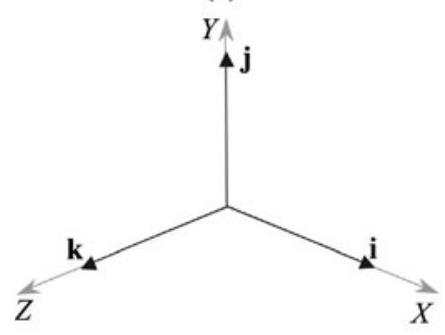
\includegraphics[max width=0.3\textwidth]{2023_01_16_a848224efad29cd66460g-065}}
    \subfigure[]{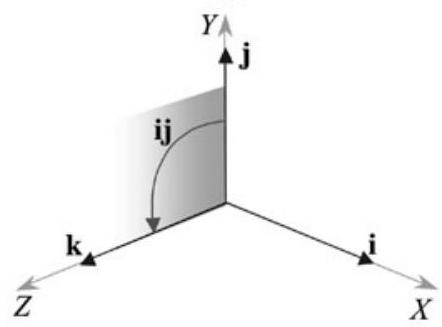
\includegraphics[max width=0.3\textwidth]{2023_01_16_a848224efad29cd66460g-065(2)}}\\
    \subfigure[]{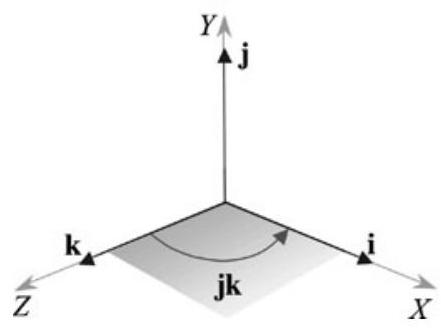
\includegraphics[max width=0.3\textwidth]{2023_01_16_a848224efad29cd66460g-065(1)}}
    \subfigure[]{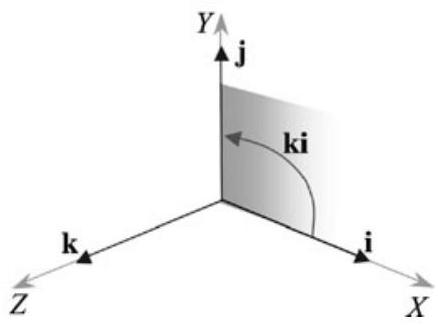
\includegraphics[max width=0.3\textwidth]{2023_01_16_a848224efad29cd66460g-065(3)}}
    \caption[short]{解释乘积$\mathbf{i j}, \mathbf{j} \mathbf{k}, \mathbf{k i}$}
\end{figure}

人们可以从两个角度来看待 Hamilton 的规则。第一,它们是结合三个虚数项的代数结果。第二,它们反映了空间的潜在几何结构。后一种解释被 P.G.Tait 采用,并在他的书《四元数概论》[21]中概述。 Tait 的方法假设三个单位向量$\mathbf{i}, \mathbf{j}, \mathbf{k}$分别与$x-, y$-, $z$-轴对齐:

\begin{CJK}{UTF8}{gkai}
    “将$\mathbf{i}$乘以$\mathbf{j}$或$\mathbf{i} \mathbf{j}$的结果被定义为$\mathbf{j}$在垂直于$\mathbf{i}$的平面上沿正方向旋转一个直角,换句话说,$\mathbf{i}$对$\mathbf{j}$的操作将其旋转,使其与$\mathbf{k}$重合;因此简单地$\mathbf{i j}=\mathbf{k}$。

    为了保持一致,必须承认,如果$\mathbf{i}$操作的不是$\mathbf{j}$,而是在平面$ yz $中操作与$\mathbf{i}$垂直的任何其他单位向量,它将使其沿同一方向旋转一个直角,因此$\mathbf{i k}$只能是$-\mathbf{j}$。

    将我们通过引用$\mathbf{i}$所说明的定义扩展到其他单位向量,很明显,$\mathbf{j}$作用于$\mathbf{k}$一定会得到$\mathbf{i}$,或$\mathbf{j} \mathbf{k}=\mathbf{i}$。”
\end{CJK}

Tait的解释见图$5.1$ (a)-(d)。图$5.1$ (a)显示了$\mathbf{i}, \mathbf{j}, \mathbf{k}$的原始对齐方式。图$5.1$ (b)显示了将$\mathbf{j}$转换为$\mathbf{k}$的效果。图$5.1$ (c)显示$\mathbf{k}$变为$\mathbf{i}$,图$5.1$ (d)显示$\mathbf{i}$变为$\mathbf{j}$。

到目前为止,我们还没有提到虚量——我们只有:
$$
\begin{array}{ll}
\mathbf{i j}=\mathbf{k}, & \mathbf{j} \mathbf{k}=\mathbf{i}, \quad \mathbf{k i}=\mathbf{j} \\
\mathbf{j} \mathbf{i}=-\mathbf{k}, & \mathbf{k j}=-\mathbf{i}, \quad \mathbf{i k}=-\mathbf{j}
\end{array}
$$

如果我们假设这些向量服从代数的分配律和结合律,它们的虚数性质就暴露出来了。例如:
$$
\mathbf{i j}=\mathbf{k}
$$

和都乘以$\mathbf{i}$:
$$
\mathbf{i}\mathbf{i} \mathbf{j}=\mathbf{i k}=-\mathbf{j}
$$

因此,
$$
\mathbf{i i}=\mathbf{i}^{2}=-1 .
$$

同样,我们可以展示$\mathbf{j}^{2}=\mathbf{k}^{2}=-1$。

接下来:
$$
\mathbf{i j k}=\mathbf{i}(\mathbf{j k})=\mathbf{i} \mathbf{i}=\mathbf{i}^{2}=-1 .
$$

因此,仅仅通过声明叉乘的作用, Hamilton 的规则就出现了,以及它们所有的虚数特征。 Tait 还提出以下看法:

\begin{CJK}{UTF8}{gkai}
    “由Servois于1813年发表在 Gergonne 的年鉴上的一篇非常奇怪的推测是迄今为止发现的唯一一篇,其中包含了四元数预测的最轻微痕迹。他力图将平面的形式$a+b \sqrt{-1}$扩展到空间中,通过类推的方法在空间中写出有向的单位线
$$
p \cos \alpha+q \cos \beta+r \cos \gamma,
$$

其中$\alpha, \beta, \gamma$是它对三个轴的倾斜度。他很容易看出$p, q, r$一定是非实数:但是,他问道:“它们是虚的可约化为一般形式$A+B \sqrt{-1}$吗?”\footnote{"seraient-elles imaginaires réductibles à la forme générale $A+B \sqrt{-1}$ ?"} 这可能不是答案。事实上,它们是四元数演算的$\mathbf{i}, \mathbf{j}, \mathbf{k}$。”
\end{CJK}

因此,法国数学家 François-Joseph Servois(1768-1847)是另一个非常接近发现四元数的人。此外,泰特和汉密尔顿显然都不知道罗德里格斯发表的论文。

而且还不止于此。杰出的德国数学家卡尔·弗里德里希·高斯(karl Friedrich Gauss, 1777-1855)非常谨慎,害怕发表任何过于革命性的东西,以防他被同行的数学家嘲笑。他的日记显示,他在尼古拉·伊万诺维奇·洛巴切夫斯基(Nikolai Ivanovich Lobachevsky)之前就预见到了非欧几里得几何。他在1819年的日记中写道,他发现了一种方法,可以求出两个四重数$(a, b, c, d)$和$(\alpha, \beta, \gamma, \delta)$的乘积:
$$
\begin{aligned}
(A, B, C, D)= & (a, b, c, d)(\alpha, \beta, \gamma, \delta) \\
= & (a \alpha-b \beta-c \gamma-d \delta, a \beta+b \alpha-c \delta+d \gamma, \\
& a \gamma+b \delta+c \alpha-d \beta, a \delta-b \gamma+c \beta+d \alpha) .
\end{aligned}
$$

乍一看,这个结果看起来不像四元数乘积,但如果我们转置四元组的第二个和第三个坐标,并将它们视为四元数,我们就有
$$
\begin{aligned}
(A, B, C, D) & =(a+c i+b j+d k)(\alpha+\gamma i+\beta j+\delta k) \\
& =a \alpha-c \gamma-b \beta-d \delta+a(\gamma i+\beta j+\delta k) \\
& =+\alpha(c i+b j+d k),(b \delta-d \beta) i+(d \gamma-c \delta) j+(c \beta-b \gamma) k
\end{aligned}
$$

这和 Hamilton 的四元数积是一样的!此外,高斯还认识到这个乘积是非交换的。然而,他并没有发表他的发现,而是让汉密尔顿为自己发明了四元数,发表了他的结果,并获得了荣誉。

1881年和1884年,耶鲁大学的乔赛亚·威拉德·吉布斯(Josiah Willard Gibbs)为他的学生打印了关于矢量分析的课堂笔记。吉布斯割断了四元数的实数部分和向量部分之间的“脐带”,并提出了三维向量作为一个独立的对象,没有任何虚数的内涵。吉布斯还采纳了德国数学家赫尔曼Günter格拉斯曼(Hermann Günter Grassmann, 1809-1877)的思想,格拉斯曼自1832年以来一直在发展他自己的向量系统思想。Gibbs还使用四元数积的相关部分定义了标量积和向量积。最后,在1901年,吉布斯的学生埃德温·比德韦尔·威尔逊(Edwin Bidwell Wilson)以书的形式出版了吉布斯的笔记:向量分析[23],其中包含了今天使用的符号。

四元数代数绝对是虚的,但仅仅通过分离向量部分并忽略虚数规则, Gibbs 就能够揭示一个新的数学分支,它爆发为向量分析。

Hamilton 和他的支持者无法说服他们的同行,四元数可以表示矢量,最终,吉布斯的符号赢得了胜利,四元数淡出了舞台。

近年来,四元数被飞行模拟行业重新发现,最近又被计算机图形社区发现,它们被用于围绕任意轴旋转向量。在这期间,许多人都有机会研究代数,并提出利用代数特性的新方法。

让我们看看四元数$q$的三种写法:
\begin{align}
q= & s+x i+y j+z k \\
q= & s+\mathbf{v} \\
q= & {[s, \mathbf{v}] } \\
& \text { where } s, x, y, z \in \mathbb{R}, \quad \mathbf{v} \in \mathbb{R}^{3} \notag\\
& \text { and } i^{2}=j^{2}=k^{2}=-1 .\notag
\end{align}

区别是相当微妙的。在(5.1)中,我们有 Hamilton 的原始定义及其虚数术语和相关规则。在(5.2)中,' $+$ '符号用于向向量添加标量,这看起来很奇怪,但却有效。在(5.3)中,我们有一个由标量和向量组成的有序对。

现在你可能会想:同一个物体怎么可能有三种不同的定义?我认为你可以随便叫一个对象,只要它们在代数上是相同的。例如,用矩阵表示法表示一组线性方程,得到的结果与日常方程相同。因此,两种表示法是同样有效的。

虽然我在其他出版物中使用了(5.1)和(5.2)中的符号,但在本书中我使用的是有序对。因此,我们需要证明的是, Hamilton 对四元数的原始定义(5.1),包括它的标量和三个虚数项,可以被一个由标量和一个“现代”向量组成的有序对(5.3)所取代。

\section{定义四元数}
让我们从两个四元数$q_{a}$和$q_{b}$ à la Hamilton开始:\footnote{译注,原句是:Let's start with two quaternions $q_{a}$ and $q_{b}$ à la Hamilton:,感觉原句有错误排过来的字符。 }


$$
\begin{aligned}
& q_{a}=s_{a}+x_{a} i+y_{a} j+z_{a} k \\
& q_{b}=s_{b}+x_{b} i+y_{b} j+z_{b} k
\end{aligned}
$$

强制性的规则是:
% and the obligatory rules:
$$
\begin{gathered}
i^{2}=j^{2}=k^{2}=i j k=-1 \\
i j=k, \quad j k=i, \quad k i=j \\
j i=-k, \quad k j=-i, \quad i k=-j .
\end{gathered}
$$

我们的目标是证明$q_{a}$和$q_{b}$也可以用有序对表示
$$
\begin{aligned}
q_{a} & =\left[s_{a}, \mathbf{a}\right] \\
q_{b} & =\left[s_{b}, \mathbf{b}\right] \quad s_{a}, s_{b} \in \mathbb{R}, \quad \mathbf{a}, \mathbf{b} \in \mathbb{R}^{3} .
\end{aligned}
$$

我使用方括号作为定义的一部分,因为括号经常用于在四元数中分隔表达式。
% I have employed square brackets as part of the definition as parentheses are often used to delimit expressions within a quaternion.

四元数乘积$q_{a} q_{b}$展开为
\begin{align}
    \begin{aligned}
        q_{a} q_{b}=\left[s_{a}, \mathbf{a}\right]\left[s_{b}, \mathbf{b}\right]= & \left(s_{a}+x_{a} i+y_{a} j+z_{a} k\right)\left(s_{b}+x_{b} i+y_{b} j+z_{b} k\right) \\
        = & \left(s_{a} s_{b}-x_{a} x_{b}-y_{a} y_{b}-z_{a} z_{b}\right) \\
        & +\left(s_{a} x_{b}+s_{b} x_{a}+y_{a} z_{b}-y_{b} z_{a}\right) i \\
        & +\left(s_{a} y_{b}+s_{b} y_{a}+z_{a} x_{b}-z_{b} x_{a}\right) j \\
        & +\left(s_{a} z_{b}+s_{b} z_{a}+x_{a} y_{b}-x_{b} y_{a}\right) k
        \end{aligned}
\end{align}

式(5.4)采用另一个四元数的形式,证实四元数乘积是封闭的。

在此阶段,Hamilton将虚数$i, j, k$转换为单位笛卡尔向量$\mathbf{i}, \mathbf{j}, \mathbf{k}$,并将(5.4)转换为向量形式。这种方法的问题是向量保留了它们的虚根。Simon Altmann的建议是将虚数替换为有序对:
$$
i=[0, \mathbf{i}] \quad j=[0, \mathbf{j}] \quad k=[0, \mathbf{k}]
$$

它们本身就是四元数,叫做四元数单位。用四元数单位定义四元数的思想与用单位笛卡尔向量定义向量的思想完全相同。此外,它允许向量在没有任何虚数关联的情况下存在。

让我们用(5.4)中的这些四元数单位和$[1,\mathbf{0}]=1$替换:
\begin{align}
    \begin{aligned}
        {\left[s_{a}, \mathbf{a}\right]\left[s_{b}, \mathbf{b}\right]=} & \left(s_{a} s_{b}-x_{a} x_{b}-y_{a} y_{b}-z_{a} z_{b}\right)[1, \mathbf{0}] \\
        & +\left(s_{a} x_{b}+s_{b} x_{a}+y_{a} z_{b}-y_{b} z_{a}\right)[0, \mathbf{i}] \\
        & +\left(s_{a} y_{b}+s_{b} y_{a}+z_{a} x_{b}-z_{b} x_{a}\right)[0, \mathbf{j}] \\
        & +\left(s_{a} z_{b}+s_{b} z_{a}+x_{a} y_{b}-x_{b} y_{a}\right)[0, \mathbf{k}] .
    \end{aligned}
\end{align}



接下来,我们使用之前定义的规则展开(5.5):
\begin{align}
    \begin{aligned}
        {\left[s_{a}, \mathbf{a}\right]\left[s_{b}, \mathbf{b}\right]=} & {\left[s_{a} s_{b}-x_{a} x_{b}-y_{a} y_{b}-z_{a} z_{b}, \mathbf{0}\right] } \\
        & +\left[0,\left(s_{a} x_{b}+s_{b} x_{a}+y_{a} z_{b}-y_{b} z_{a}\right) \mathbf{i}\right] \\
        & +\left[0,\left(s_{a} y_{b}+s_{b} y_{a}+z_{a} x_{b}-z_{b} x_{a}\right) \mathbf{j}\right] \\
        & +\left[0,\left(s_{a} z_{b}+s_{b} z_{a}+x_{a} y_{b}-x_{b} y_{a}\right) \mathbf{k}\right] .
    \end{aligned} 
\end{align}

(5.6)的垂直扫描显示了一些隐藏的向量:
\begin{align}
    \begin{aligned}
        {\left[s_{a}, \mathbf{a}\right]\left[s_{b}, \mathbf{b}\right]=} & {\left[s_{a} s_{b}-x_{a} x_{b}-y_{a} y_{b}-z_{a} z_{b}, \mathbf{0}\right] } \\
        & +\left[0, s_{a}\left(x_{b} \mathbf{i}+y_{b} \mathbf{j}+z_{b} \mathbf{k}\right)+s_{b}\left(x_{a} \mathbf{i}+y_{a} \mathbf{j}+z_{a} \mathbf{k}\right)\right. \\
        & \left.+\left(y_{a} z_{b}-y_{b} z_{a}\right) \mathbf{i}+\left(z_{a} x_{b}-z_{b} x_{a}\right) \mathbf{j}+\left(x_{a} y_{b}-x_{b} y_{a}\right) \mathbf{k}\right] .
    \end{aligned}
\end{align}

式(5.7)包含两个有序对,现在可以组合:
\begin{align}
    \begin{aligned}
        {\left[s_{a}, \mathbf{a}\right]\left[s_{b}, \mathbf{b}\right]=} & {\left[s_{a} s_{b}-x_{a} x_{b}-y_{a} y_{b}-z_{a} z_{b},\right.} \\
        & s_{a}\left(x_{b} \mathbf{i}+y_{b} \mathbf{j}+z_{b} \mathbf{k}\right)+s_{b}\left(x_{a} \mathbf{i}+y_{a} \mathbf{j}+z_{a} \mathbf{k}\right) \\
        & \left.+\left(y_{a} z_{b}-y_{b} z_{a}\right) \mathbf{i}+\left(z_{a} x_{b}-z_{b} x_{a}\right) \mathbf{j}+\left(x_{a} y_{b}-x_{b} y_{a}\right) \mathbf{k}\right] .
    \end{aligned}
\end{align}

如果我们令
$$
\begin{aligned}
& \mathbf{a}=x_{a} \mathbf{i}+y_{a} \mathbf{j}+z_{a} \mathbf{k} \\
& \mathbf{b}=x_{b} \mathbf{i}+y_{b} \mathbf{j}+z_{b} \mathbf{k}
\end{aligned}
$$

代入(5.8)得到:
\begin{align}
    \left[s_{a}, \mathbf{a}\right]\left[s_{b}, \mathbf{b}\right]=\left[s_{a} s_{b}-\mathbf{a} \cdot \mathbf{b}, s_{a} \mathbf{b}+s_{b} \mathbf{a}+\mathbf{a} \times \mathbf{b}\right]
\end{align}

它定义了四元数乘积。

从现在开始,我们不必担心 Hamilton 的规则,因为它们嵌入在(5.9)中。此外,我们的向量没有虚数的关联。

虽然Rodrigues没有使用(5.9)中使用的Gibbs向量符号,但他设法计算出等效的代数表达式,这是一项成就。

\subsection{四元数单位}
使用(5.9),我们可以通过对四元数单位进行平方来检查四元数单位是否为虚数:
$$
\begin{aligned}
i & =[0, \mathbf{i}] \\
i^{2} & =[0, \mathbf{i}][0, \mathbf{i}] \\
& =[\mathbf{i} \cdot \mathbf{i}, \mathbf{i} \times \mathbf{i}] \\
& =[-1, \mathbf{0}]
\end{aligned}
$$

这是一个实数四元数,等价于$-1$,确认$[0,\mathbf{i}]$是虚数。使用类似的展开,我们可以显示$[0,\mathbf{j}]$和$[0,\mathbf{k}]$具有相同的属性。

现在让我们计算$i j, jk $和$k i$的乘积:
$$
\begin{aligned}
i j & =[0, \mathbf{i}][0, \mathbf{j}] \\
& =[-\mathbf{i} \cdot \mathbf{j}, \mathbf{i} \times \mathbf{j}] \\
& =[0, \mathbf{k}]
\end{aligned}
$$

就是四元数单位$k$。
$$
\begin{aligned}
j k & =[0, \mathbf{j}][0, \mathbf{k}] \\
& =[-\mathbf{j} \cdot \mathbf{k}, \mathbf{j} \times \mathbf{k}] \\
& =[0, \mathbf{i}]
\end{aligned}
$$

就是四元数单位$i$。
$$
\begin{aligned}
k i & =[0, \mathbf{k}][0, \mathbf{i}] \\
& =[-\mathbf{k} \cdot \mathbf{i}, \mathbf{k} \times \mathbf{i}] \\
& =[0, \mathbf{j}]
\end{aligned}
$$

就是四元数单位$j$。

接下来,让我们确认$i j k=-1$:
$$
\begin{aligned}
i j k & =[0, \mathbf{i}][0, \mathbf{j}][0, \mathbf{k}] \\
& =[0, \mathbf{k}][0, \mathbf{k}] \\
& =[-\mathbf{k} \cdot \mathbf{k}, \mathbf{k} \times \mathbf{k}] \\
& =[-1, \mathbf{0}]
\end{aligned}
$$

这是一个四元数,相当于$-1$,确认$ ij k=-1$。

因此,有序对的表示法符合 Hamilton 的所有规则。然而,最后一个双积假设四元数是结合的。因此,让我们再次检查,以显示$(i j) k=i(j k)$:
$$
\begin{aligned}
i(j k) & =[0, \mathbf{i}][0, \mathbf{j}][0, \mathbf{k}] \\
& =[0, \mathbf{i}][0, \mathbf{i}] \\
& =[-\mathbf{i} \cdot \mathbf{i}, \mathbf{i} \times \mathbf{i}] \\
& =[-1, \mathbf{0}]
\end{aligned}
$$

这是正确的。

\subsection{四元数乘积的例子}
尽管我们还没有发现四元数是如何用于旋转向量的,让我们通过评估一个例子来集中讨论它们的代数特征。
$$
\begin{aligned}
& q_{a}=[1,2 \mathbf{i}+3 \mathbf{j}+4 \mathbf{k}] \\
& q_{b}=[2,3 \mathbf{i}+4 \mathbf{j}+5 \mathbf{k}]
\end{aligned}
$$

$q_{a} q_{b}$的乘积是
$$
\begin{aligned}
q_{a} q_{b}= & {[1,2 \mathbf{i}+3 \mathbf{j}+4 \mathbf{k}][2,3 \mathbf{i}+4 \mathbf{j}+5 \mathbf{k}] } \\
= & {[1 \times 2-(2 \times 3+3 \times 4+4 \times 5),} \\
& 1(3 \mathbf{i}+4 \mathbf{j}+5 \mathbf{k})+2(2 \mathbf{i}+3 \mathbf{j}+4 \mathbf{k}) \\
& +(3 \times 5-4 \times 4) \mathbf{i}-(2 \times 5-4 \times 3) \mathbf{j}+(2 \times 4-3 \times 3) \mathbf{k}] \\
= & {[-36,7 \mathbf{i}+10 \mathbf{j}+13 \mathbf{k}-\mathbf{i}+2 \mathbf{j}-\mathbf{k}] } \\
= & {[-36,6 \mathbf{i}+12 \mathbf{j}+12 \mathbf{k}] }
\end{aligned}
$$

这是另一个表示四元数的有序对。

在证明了Hamilton的虚数表示法有一个向量等价,并且可以表示为一个有序对之后,我们继续使用这个表示法并描述四元数的其他特征。请注意,我们可以放弃Hamilton规则,因为它们嵌入在四元数乘积的定义中,并将在以下定义中出现。

\section{代数的定义}
四元数是有序对:
$$
q=[s, \mathbf{v}] \quad s \in \mathbb{R}, \mathbf{v} \in \mathbb{R}^{3} .
$$

如果我们用$\mathbf{v}$的分量来表示它,我们有
$$
q=[s, x \mathbf{i}+y \mathbf{j}+z \mathbf{k}] \quad s, x, y, z \in \mathbb{R} .
$$

\section{四元数加减法}
加减法使用以下法则:
$$
\begin{aligned}
q_{a} & =\left[s_{a}, \mathbf{a}\right] \\
q_{b} & =\left[s_{b}, \mathbf{b}\right] \\
q_{a} \pm q_{b} & =\left[s_{a} \pm s_{b}, \mathbf{a} \pm \mathbf{b}\right]
\end{aligned}
$$

示例:
$$
\begin{aligned}
q_{a} & =[0.5,2 \mathbf{i}+3 \mathbf{j}-4 \mathbf{k}] \\
q_{b} & =[0.1,4 \mathbf{i}+5 \mathbf{j}+6 \mathbf{k}] \\
q_{a}+q_{b} & =[0.6,6 \mathbf{i}+8 \mathbf{j}+2 \mathbf{k}] \\
q_{a}-q_{b} & =[0.4,-2 \mathbf{i}-2 \mathbf{j}-10 \mathbf{k}] .
\end{aligned}
$$

\section{实四元数}
实四元数有一个零向量项:
$$
q=[s, \mathbf{0}]
$$

两个实四元数的乘积是
$$
\begin{aligned}
q_{a} & =\left[s_{a}, \mathbf{0}\right] \\
q_{b} & =\left[s_{b}, \mathbf{0}\right] \\
q_{a} q_{b} & =\left[s_{a}, \mathbf{0}\right]\left[s_{b}, \mathbf{0}\right] \\
& =\left[s_{a} s_{b}, \mathbf{0}\right]
\end{aligned}
$$

这是另一个实数四元数,表明它们的行为就像实数一样:
$$
[s, \mathbf{0}] \equiv s .
$$

我们已经遇到过包含零虚数项的复数:
$$
a+b i=a \quad \text { 当 } b=0 .
$$

\section{四元数乘以标量}
直觉表明,四元数乘以一个标量应该遵循以下规则:
$$
\begin{aligned}
q & =[s, \mathbf{v}] \\
\lambda q & =\lambda[s, \mathbf{v}] \quad \lambda \in \mathbb{R} \\
& =[\lambda s, \lambda \mathbf{v}] .
\end{aligned}
$$

我们可以用一个四元数乘以一个实四元数形式的标量来证实我们的直觉:
$$
\begin{aligned}
q & =[s, \mathbf{v}] \\
\lambda & =[\lambda, \mathbf{0}] \\
\lambda q & =[\lambda, \mathbf{0}][s, \mathbf{v}] \\
& =[\lambda s, \lambda \mathbf{v}]
\end{aligned}
$$

这是很好的证明。

\section{纯四元数}
Hamilton将纯四元数定义为具有零标量项的四元数:
$$
q=x i+y j+z k
$$

它只是一个“矢量”,有它所有虚数的特性。然而,Simon Altmann和其他人认为,Hamilton把实数为零的四元数称为向量,这是一个严重的错误。

主要问题是有两种类型的向量:极坐标和轴坐标,也称为伪向量。理查德·费曼(Richard Feynman)将极向量描述为“诚实的”向量[12],并表示有向线的日常向量。然而,轴向量是从极向量计算出来的,例如在向量积中。然而,这两种类型的向量在变换时行为并不相同。例如,给定两个“诚实的”极坐标向量$\mathbf{a}$和$\mathbf{b}$,我们可以计算轴向量:$\mathbf{c}=\mathbf{a} \times\mathbf{b}$。接下来,如果我们将$\mathbf{a}$和$\mathbf{b}$赋值到原点的反转变换,使$\mathbf{a}$变为$-\mathbf{a}$, $\mathbf{b}$变为$-\mathbf{b}$,并计算它们的叉乘$(-\mathbf{a}) \times(-\mathbf{b})$,我们仍然得到$\mathbf{c}$ !这意味着轴向量$\mathbf{c}$不能与$\mathbf{a}$和$\mathbf{b}$一起转换。

可以认为,逆变换不是一个“适当的”变换,因为它把一个右手轴集变成了一个左手轴集。但在物理学中,自然定律在这两种系统中都适用。不幸的是,Hamilton并没有意识到这种区别,因为他刚刚发明了向量。然而,在过去的几年里,Hamilton的四元数向量显然是一个轴向量,而不是一个极向量。

正如我们将看到的,在三维旋转中,四元数采用这种形式
$$
q=\left[\cos \frac{1}{2} \theta, \sin \frac{1}{2} \theta \mathbf{v}\right]
$$

其中$\theta$是旋转角度,$\mathbf{v}$是旋转轴,当我们设置$\theta=180^{\circ}$时,我们得到
$$
q=[0, \mathbf{v}]
$$

which remains a quaternion, even though it only contains a vector part. Consequently, we define a pure quaternion as

$$
q=[0, \mathbf{v}]
$$

The product of two pure quaternions is

$$
\begin{aligned}
q_{a} & =[0, \mathbf{a}] \\
q_{b} & =[0, \mathbf{b}] \\
q_{a} q_{b} & =[0, \mathbf{a}][0, \mathbf{b}] \\
& =[-\mathbf{a} \cdot \mathbf{b}, \mathbf{a} \times \mathbf{b}]
\end{aligned}
$$

which is no longer 'pure', as some of the original vector information has 'tunnelled' across into the real part via the dot product.

\section{单位四元数}
Let's pursue this analysis further by introducing some familiar vector notation.

Give vector $\mathbf{v}$, then

$$
\mathbf{v}=v \hat{\mathbf{v}} \quad \text { where } v=|\mathbf{v}|, \text { and }|\hat{\mathbf{v}}|=1 .
$$

Combining this with the definition of a pure quaternion we get:

$$
\begin{aligned}
q & =[0, \mathbf{v}] \\
& =[0, v \hat{\mathbf{v}}] \\
& =v[0, \hat{\mathbf{v}}]
\end{aligned}
$$

and reveals the object $[0, \hat{\mathbf{v}}]$ which is called the unit quaternion and comprises a zero scalar and a unit vector. It is convenient to identify this unit quaternion as $\hat{q}$ :

$$
\hat{q}=[0, \hat{\mathbf{v}}]
$$

So now we have a notation similar to that of vectors where a vector $\mathbf{v}$ is described in terms of its unit form:

$$
\mathbf{v}=v \hat{\mathbf{v}}
$$

and a quaternion $q$ is also described in terms of its unit form:

$$
q=v \hat{q} .
$$

Note that $\hat{q}$ is an imaginary object as it squares to $-1$ :

$$
\begin{aligned}
\hat{q}^{2} & =[0, \hat{\mathbf{v}}][0, \hat{\mathbf{v}}] \\
& =[-\hat{\mathbf{v}} \cdot \hat{\mathbf{v}}, \hat{\mathbf{v}} \times \hat{\mathbf{v}}] \\
& =[-1, \mathbf{0}] \\
& =-1
\end{aligned}
$$

which is not too surprising, bearing in mind Hamilton's original invention!

\section{四元数的加法形式}
We now come to the idea of splitting a quaternion into its constituent parts: a real quaternion and a pure quaternion. Again, intuition suggests that we can write a quaternion as

$$
\begin{aligned}
q & =[s, \mathbf{v}] \\
& =[s, \mathbf{0}]+[0, \mathbf{v}]
\end{aligned}
$$

and we can test this by forming the algebraic product of two quaternions represented in this way:

$$
\begin{aligned}
q_{a} & =\left[s_{a}, \mathbf{0}\right]+[0, \mathbf{a}] \\
q_{b} & =\left[s_{b}, \mathbf{0}\right]+[0, \mathbf{b}] \\
q_{a} q_{b} & =\left(\left[s_{a}, \mathbf{0}\right]+[0, \mathbf{a}]\right)\left(\left[s_{b}, \mathbf{0}\right]+[0, \mathbf{b}]\right) \\
& =\left[s_{a}, \mathbf{0}\right]\left[s_{b}, \mathbf{0}\right]+\left[s_{a}, \mathbf{0}\right][0, \mathbf{b}]+[0, \mathbf{a}]\left[s_{b}, \mathbf{0}\right]+[0, \mathbf{a}][0, \mathbf{b}] \\
& =\left[s_{a} s_{b}, \mathbf{0}\right]+\left[0, s_{a} \mathbf{b}\right]+\left[0, s_{b} \mathbf{a}\right]+[-\mathbf{a} \cdot \mathbf{b}, \mathbf{a} \times \mathbf{b}] \\
& =\left[s_{a} s_{b}-\mathbf{a} \cdot \mathbf{b}, s_{a} \mathbf{b}+s_{b} \mathbf{a}+\mathbf{a} \times \mathbf{b}\right]
\end{aligned}
$$

which is correct, and confirms that the additive form works.

\section{四元数的二进制形式}
Having shown that the additive form of a quaternion works, and discovered the unit quaternion, we can join the two objects together as follows:

$$
\begin{aligned}
q & =[s, \mathbf{v}] \\
& =[s, \mathbf{0}]+[0, \mathbf{v}] \\
& =[s, \mathbf{0}]+v[0, \hat{\mathbf{v}}] \\
& =s+v \hat{q}
\end{aligned}
$$

Just to recap, $s$ is a scalar, $v$ is the length of the vector term, and $\hat{q}$ is the unit quaternion $[0, \hat{\mathbf{v}}]$.

Look how similar this notation is to a complex number:

$$
\begin{aligned}
& z=a+b i \\
& q=s+v \hat{q}
\end{aligned}
$$

where $a, b, s, v$ are scalars, $i$ is the unit imaginary and $\hat{q}$ is the unit quaternion.

\section{共轭}
We have already discovered that the conjugate of a complex number $z=a+b \mathrm{i}$ is given by

$$
z^{*}=a-b \mathrm{i}
$$

and is very useful in computing the inverse of $z$. The quaternion conjugate plays a similar role in computing the inverse of a quaternion. Therefore, given

$$
q=[s, \mathbf{v}]
$$

the quaternion conjugate is defined as

$$
q^{*}=[s,-\mathbf{v}] .
$$

If we compute the product $q q^{*}$ we obtain

$$
\begin{aligned}
q q^{*} & =[s, \mathbf{v}][s,-\mathbf{v}] \\
& =\left[s^{2}-\mathbf{v} \cdot(-\mathbf{v}),-s \mathbf{v}+s \mathbf{v}+\mathbf{v} \times(-\mathbf{v})\right] \\
& =\left[s^{2}+\mathbf{v} \cdot \mathbf{v}, \mathbf{0}\right] \\
& =\left[s^{2}+v^{2}, \mathbf{0}\right] .
\end{aligned}
$$

Let's show that $q q^{*}=q^{*} q$ :

$$
\begin{aligned}
q^{*} q & =[s,-\mathbf{v}][s, \mathbf{v}] \\
& =\left[s^{2}-(-\mathbf{v}) \cdot \mathbf{v}, s \mathbf{v}-s \mathbf{v}+(-\mathbf{v}) \times \mathbf{v}\right] \\
& =\left[s^{2}+\mathbf{v} \cdot \mathbf{v}, \mathbf{0}\right] \\
& =\left[s^{2}+v^{2}, \mathbf{0}\right] \\
& =q q^{*} .
\end{aligned}
$$

Now let's show that $\left(q_{a} q_{b}\right)^{*}=q_{b}^{*} q_{a}^{*}$.

$$
\begin{aligned}
q_{a} & =\left[s_{a}, \mathbf{a}\right] \\
q_{b} & =\left[s_{b}, \mathbf{b}\right] \\
q_{a} q_{b} & =\left[s_{a}, \mathbf{a}\right]\left[s_{b}, \mathbf{b}\right] \\
& =\left[s_{a} s_{b}-\mathbf{a} \cdot \mathbf{b}, s_{a} \mathbf{b}+s_{b} \mathbf{a}+\mathbf{a} \times \mathbf{b}\right] \\
\left(q_{a} q_{b}\right)^{*} & =\left[s_{a} s_{b}-\mathbf{a} \cdot \mathbf{b},-s_{a} \mathbf{b}-s_{b} \mathbf{a}-\mathbf{a} \times \mathbf{b}\right] .
\end{aligned}
$$

Next, we compute $q_{b}^{*} q_{a}^{*}$

$$
\begin{aligned}
q_{a}^{*} & =\left[s_{a},-\mathbf{a}\right] \\
q_{b}^{*} & =\left[s_{b},-\mathbf{b}\right] \\
q_{b}^{*} q_{a}^{*} & =\left[s_{b},-\mathbf{b}\right]\left[s_{a},-\mathbf{a}\right] \\
& =\left[s_{a} s_{b}-\mathbf{a} \cdot \mathbf{b},-s_{a} \mathbf{b}-s_{b} \mathbf{a}-\mathbf{a} \times \mathbf{b}\right] .
\end{aligned}
$$

And as (5.10) equals $(5.11),\left(q_{a} q_{b}\right)^{*}=q_{b}^{*} q_{a}^{*}$.

\section{四元数范数}
The norm of a complex number $z=a+b i$ is defined as

$$
|z|=\sqrt{a^{2}+b^{2}}
$$

which allows us to write

$$
z z^{*}=|z|^{2} \text {. }
$$

Similarly, the norm of a quaternion $q=[s, \mathbf{v}]$ is defined as

$$
|q|=\sqrt{s^{2}+v^{2}}
$$

where $v=|\mathbf{v}|$ which allows us to write

$$
q q^{*}=|q|^{2} .
$$

For example, given

$$
\begin{aligned}
q & =[1,4 \mathbf{i}+4 \mathbf{j}-4 \mathbf{k}] \\
|q| & =\sqrt{1^{2}+4^{2}+4^{2}+(-4)^{2}} \\
& =\sqrt{49} \\
& =7 .
\end{aligned}
$$

\section{归一化四元数}
A quaternion with a unit norm is called a normalised quaternion. For example, the quaternion $q=[s, \mathbf{v}]$ is normalised by dividing it by $|q|$ :

$$
q^{\prime}=\frac{q}{\sqrt{s^{2}+v^{2}}} .
$$

We must be careful not to confuse the unit quaternion with a unit-norm quaternion. The unit quaternion is $[0, \hat{\mathbf{v}}]$ with a unit-vector part, whereas a unit-norm quaternion is normalised such that $s^{2}+v^{2}=1$.

I will be careful to distinguish between these two terms as many authorsincluding myself-use the term unit quaternion to describe a quaternion with a unit norm. For example

$$
q=[1,4 \mathbf{i}+4 \mathbf{j}-4 \mathbf{k}]
$$

has a norm of 7 , and $q$ is normalised by dividing by 7 :

$$
q^{\prime}=\frac{1}{7}[1,4 \mathbf{i}+4 \mathbf{j}-4 \mathbf{k}] .
$$

The type of unit-norm quaternion we will be using takes the form:

$$
q=\left[\cos \frac{1}{2} \theta, \sin \frac{1}{2} \theta \hat{\mathbf{v}}\right]
$$

because $\cos ^{2} \theta+\sin ^{2} \theta=1$

\section{四元数乘积}
Having shown that ordered pairs can represent a quaternion and its various manifestations, let's summarise the products we will eventually encounter. To start, we have the product of two normal quaternions:

$$
\begin{aligned}
q_{a} q_{b} & =\left[s_{a}, \mathbf{a}\right]\left[s_{b}, \mathbf{b}\right] \\
& =\left[s_{a} s_{b}-\mathbf{a} \cdot \mathbf{b}, s_{a} \mathbf{b}+s_{b} \mathbf{a}+\mathbf{a} \times \mathbf{b}\right] .
\end{aligned}
$$

\subsection{纯四元数的乘积}
Given two pure quaternions:

$$
\begin{aligned}
& q_{a}=[0, \mathbf{a}] \\
& q_{b}=[0, \mathbf{b}]
\end{aligned}
$$

their product is

$$
\begin{aligned}
q_{a} q_{b} & =[0, \mathbf{a}][0, \mathbf{b}] \\
& =[-\mathbf{a} \cdot \mathbf{b}, \mathbf{a} \times \mathbf{b}] .
\end{aligned}
$$

\subsection{两个单位范数四元数的乘积}
Given two unit-norm quaternions:

$$
\begin{aligned}
q_{a} & =\left[s_{a}, \mathbf{a}\right] \\
q_{b} & =\left[s_{b}, \mathbf{b}\right]
\end{aligned}
$$

where $\left|q_{a}\right|=\left|q_{b}\right|=1$. Their product is another unit-norm quaternion, which is proved as follows.

We assume $q_{c}=\left[s_{c}, \mathbf{c}\right]$ and show that $\left|q_{c}\right|=s_{c}^{2}+c^{2}=1$ where

$$
\begin{aligned}
{\left[s_{c}, \mathbf{c}\right] } & =\left[s_{a}, \mathbf{a}\right]\left[s_{b}, \mathbf{b}\right] \\
& =\left[s_{a} s_{b}-\mathbf{a} \cdot \mathbf{b}, s_{a} \mathbf{b}+s_{b} \mathbf{a}+\mathbf{a} \times \mathbf{b}\right] .
\end{aligned}
$$

Let's assume the angle between $\mathbf{a}$ and $\mathbf{b}$ is $\theta$, which permits us to write

$$
\begin{aligned}
s_{c} & =s_{a} s_{b}-a b \cos \theta \\
\mathbf{c} & =s_{a} b \hat{\mathbf{b}}+s_{b} a \hat{\mathbf{a}}+a b \sin \theta(\hat{\mathbf{a}} \times \hat{\mathbf{b}}) .
\end{aligned}
$$

Therefore,

$$
\begin{aligned}
s_{c}^{2} & =\left(s_{a} s_{b}-a b \cos \theta\right)\left(s_{a} s_{b}-a b \cos \theta\right) \\
& =s_{a}^{2} s_{b}^{2}-2 s_{a} s_{b} a b \cos \theta+a^{2} b^{2} \cos ^{2} \theta .
\end{aligned}
$$

Fig. 5.2 Geometry for $s_{a} b \hat{\mathbf{b}}+s_{b} a \hat{\mathbf{a}}+a b \sin \theta(\hat{\mathbf{a}} \times \hat{\mathbf{b}})$

\begin{center}
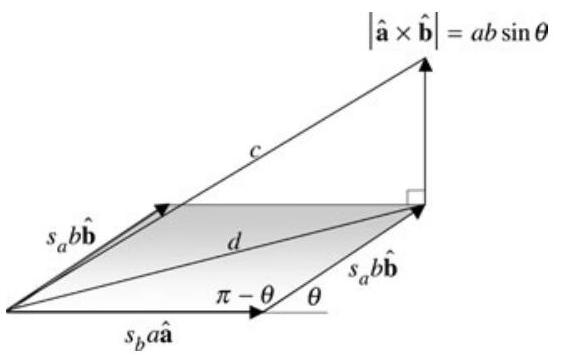
\includegraphics[max width=\textwidth]{2023_01_16_a848224efad29cd66460g-079}
\end{center}

Figure $5.2$ shows the geometry representing c.

$$
\begin{aligned}
d^{2}= & s_{b}^{2} a^{2}+s_{a}^{2} b^{2}-2 s_{a} s_{b} a b \cos (\pi-\theta) \\
= & s_{b}^{2} a^{2}+s_{a}^{2} b^{2}+2 s_{a} s_{b} a b \cos \theta \\
c^{2}= & d^{2}+a^{2} b^{2} \sin ^{2} \theta \\
= & s_{b}^{2} a^{2}+s_{a}^{2} b^{2}+2 s_{a} s_{b} a b \cos \theta+a^{2} b^{2} \sin ^{2} \theta \\
s_{c}^{2}+c^{2}= & s_{a}^{2} s_{b}^{2}-2 s_{a} s_{b} a b \cos \theta+a^{2} b^{2} \cos ^{2} \theta+s_{b}^{2} a^{2}+s_{a}^{2} b^{2}+2 s_{a} s_{b} a b \cos \theta \\
& +a^{2} b^{2} \sin ^{2} \theta \\
= & s_{a}^{2} s_{b}^{2}+a^{2} b^{2}+s_{b}^{2} a^{2}+s_{a}^{2} b^{2} \\
= & s_{a}^{2}\left(s_{b}^{2}+b^{2}\right)+a^{2}\left(s_{b}^{2}+b^{2}\right) \\
= & s_{a}^{2}+a^{2} \\
= & 1 .
\end{aligned}
$$

Therefore, the product of two unit-norm quaternions is another unit-norm quaternion. Consequently, multiplying a quaternion by a unit-norm quaternion, does not change its norm:

$$
\begin{aligned}
q_{a} & =\left[s_{a}, \mathbf{a}\right] \\
\left|q_{a}\right| & =1 \\
q_{b} & =\left[s_{b}, \mathbf{b}\right] \\
\left|q_{a} q_{b}\right| & =\left|q_{b}\right| .
\end{aligned}
$$

\subsection{四元数平方}
The square of a quaternion is given by

$$
\begin{aligned}
q & =[s, \mathbf{v}] \\
q^{2} & =[s, \mathbf{v}][s, \mathbf{v}] \\
& =\left[s^{2}-\mathbf{v} \cdot \mathbf{v}, 2 s \mathbf{v}+\mathbf{v} \times \mathbf{v}\right] \\
& =\left[s^{2}-\mathbf{v} \cdot \mathbf{v}, 2 s \mathbf{v}\right] \\
& =\left[s^{2}-x^{2}-y^{2}-z^{2}, 2 s(x \mathbf{i}+y \mathbf{j}+z \mathbf{k})\right] .
\end{aligned}
$$

For example:

$$
\begin{aligned}
q & =[7,2 \mathbf{i}+3 \mathbf{j}+4 \mathbf{k}] \\
q^{2} & =\left[7^{2}-2^{2}-3^{2}-4^{2}, 14(2 \mathbf{i}+3 \mathbf{j}+4 \mathbf{k})\right] \\
& =[20,28 \mathbf{i}+42 \mathbf{j}+56 \mathbf{k}] .
\end{aligned}
$$

The square of a pure quaternion is

$$
\begin{aligned}
q & =[0, \mathbf{v}] \\
q^{2} & =[0, \mathbf{v}][0, \mathbf{v}] \\
& =[0-\mathbf{v} \cdot \mathbf{v}, \mathbf{v} \times \mathbf{v}] \\
& =[0-\mathbf{v} \cdot \mathbf{v}, \mathbf{0}] \\
& =\left[-\left(x^{2}+y^{2}+z^{2}\right), \mathbf{0}\right]
\end{aligned}
$$

which makes the square of a pure, unit-norm quaternion equal to $-1$, and was one of the results, to which some 19 th-century mathematicians objected.

\subsection{四元数乘积的范数}
In proving that the product of two unit-norm quaternions is another unit-norm quaternion we saw that

$$
\begin{aligned}
q_{a} & =\left[s_{a}, \mathbf{a}\right] \\
q_{b} & =\left[s_{b}, \mathbf{b}\right] \\
q_{c} & =q_{a} q_{b} \\
\left|q_{c}\right|^{2} & =s_{a}^{2}\left(s_{b}^{2}+b^{2}\right)+a^{2}\left(s_{b}^{2}+b^{2}\right) \\
& =\left(s_{a}^{2}+a^{2}\right)\left(s_{b}^{2}+b^{2}\right)
\end{aligned}
$$

which, if we ignore the constraint of unit-norm quaternions, shows that the norm of a quaternion product equals the product of the individual norms:

$$
\begin{aligned}
\left|q_{a} q_{b}\right|^{2} & =\left|q_{a}\right|^{2}\left|q_{b}\right|^{2} \\
\left|q_{a} q_{b}\right| & =\left|q_{a}\right|\left|q_{b}\right|
\end{aligned}
$$

\section{逆四元数}
An important feature of quaternion algebra is the ability to divide two quaternions $q_{b} / q_{a}$, as long as $q_{a}$ does not vanish.

By definition, the inverse $q^{-1}$ of $q$ satisfies

$$
q q^{-1}=[1, \mathbf{0}]=1
$$

To isolate $q^{-1}$, we multiply (5.12) by $q^{*}$

$$
\begin{aligned}
& q^{*} q q^{-1}=q^{*} \\
& |q|^{2} q^{-1}=q^{*}
\end{aligned}
$$

and from (5.13) we can write

$$
q^{-1}=\frac{q^{*}}{|q|^{2}}
$$

If $q$ is a unit-norm quaternion, then

$$
q^{-1}=q^{*}
$$

which is useful in the context of rotations.

Furthermore, as

$$
\left(q_{a} q_{b}\right)^{*}=q_{b}^{*} q_{a}^{*}
$$

then

$$
\left(q_{a} q_{b}\right)^{-1}=q_{b}^{-1} q_{a}^{-1}
$$

Note that $q q^{-1}=q^{-1} q$

$$
\begin{aligned}
& q q^{-1}=\frac{q q^{*}}{|q|^{2}}=1 \\
& q^{-1} q=\frac{q^{*} q}{|q|^{2}}=1
\end{aligned}
$$

Thus, we represent the quotient $q_{b} / q_{a}$ as

$$
\begin{aligned}
q_{c} & =\frac{q_{b}}{q_{a}} \\
& =q_{b} q_{a}^{-1} \\
& =\frac{q_{b} q_{a}^{*}}{\left|q_{a}\right|^{2}}
\end{aligned}
$$

For completeness let's evaluate the inverse of $q$ where

$$
\begin{aligned}
q & =\left[1, \frac{1}{\sqrt{3}} \mathbf{i}+\frac{1}{\sqrt{3}} \mathbf{j}+\frac{1}{\sqrt{3}} \mathbf{k}\right] \\
q^{*} & =\left[1,-\frac{1}{\sqrt{3}} \mathbf{i}-\frac{1}{\sqrt{3}} \mathbf{j}-\frac{1}{\sqrt{3}} \mathbf{k}\right] \\
|q|^{2} & =1+\frac{1}{3}+\frac{1}{3}+\frac{1}{3}=2 \\
q^{-1}=\frac{q^{*}}{|q|^{2}} & =\frac{1}{2}\left[1,-\frac{1}{\sqrt{3}} \mathbf{i}-\frac{1}{\sqrt{3}} \mathbf{j}-\frac{1}{\sqrt{3}} \mathbf{k}\right]
\end{aligned}
$$

It should be clear that $q^{-1} q=1$ :

$$
\begin{aligned}
q^{-1} q & =\frac{1}{2}\left[1,-\frac{1}{\sqrt{3}} \mathbf{i}-\frac{1}{\sqrt{3}} \mathbf{j}-\frac{1}{\sqrt{3}} \mathbf{k}\right]\left[1, \frac{1}{\sqrt{3}} \mathbf{i}+\frac{1}{\sqrt{3}} \mathbf{j}+\frac{1}{\sqrt{3}} \mathbf{k}\right] \\
& =\frac{1}{2}\left[1+\frac{1}{3}+\frac{1}{3}+\frac{1}{3}, \mathbf{0}\right] \\
& =1 .
\end{aligned}
$$

\section{矩阵}
Matrices provide another way to express a quaternion product. For convenience, let's repeat (5.8) again and show it in matrix form:

$$
\begin{aligned}
{\left[s_{a}, \mathbf{a}\right]\left[s_{b}, \mathbf{b}\right]=} & {\left[s_{a} s_{b}-x_{a} x_{b}-y_{a} y_{b}-z_{a} z_{b},\right.} \\
& s_{a}\left(x_{b} \mathbf{i}+y_{b} \mathbf{j}+z_{b} \mathbf{k}\right)+s_{b}\left(x_{a} \mathbf{i}+y_{a} \mathbf{j}+z_{a} \mathbf{k}\right) \\
& \left.+\left(y_{a} z_{b}-y_{b} z_{a}\right) \mathbf{i}+\left(z_{a} x_{b}-z_{b} x_{a}\right) \mathbf{j}+\left(x_{a} y_{b}-x_{b} y_{a}\right) \mathbf{k}\right] \\
= & {\left[\begin{array}{cccc}
s_{a} & -x_{a} & -y_{a} & -z_{a} \\
x_{a} & s_{a} & -z_{a} & y_{a} \\
y_{a} & z_{a} & s_{a} & -x_{a} \\
z_{a} & -y_{a} & x_{a} & s_{a}
\end{array}\right]\left[\begin{array}{c}
s_{b} \\
x_{b} \\
y_{b} \\
z_{b}
\end{array}\right] . }
\end{aligned}
$$

Let's recompute the product $q_{a} q_{b}$ using the above matrix:

$$
\begin{aligned}
q_{a} & =[1,2 \mathbf{i}+3 \mathbf{j}+4 \mathbf{k}] \\
q_{b} & =[2,3 \mathbf{i}+4 \mathbf{j}+5 \mathbf{k}] \\
q_{a} q_{b} & =\left[\begin{array}{cccc}
1 & -2 & -3 & -4 \\
2 & 1 & -4 & 3 \\
3 & 4 & 1 & -2 \\
4 & -3 & 2 & 1
\end{array}\right]\left[\begin{array}{l}
2 \\
3 \\
4 \\
5
\end{array}\right] \\
& =\left[\begin{array}{c}
-36 \\
6 \\
12 \\
12
\end{array}\right] \\
& =[-36,6 \mathbf{i}+12 \mathbf{j}+12 \mathbf{k}] .
\end{aligned}
$$

\subsection{正交矩阵}
We can demonstrate that the unit-norm quaternion matrix is orthogonal by showing that the product with its transpose equals the identity matrix. As we are dealing with matrices, $\mathbf{Q}$ will represent the matrix for $q$ :

$$
\begin{aligned}
& q=[s, x \mathbf{i}+y \mathbf{j}+z \mathbf{k}] \quad \text { where } 1=s^{2}+x^{2}+y^{2}+z^{2} \\
& \mathbf{Q}=\left[\begin{array}{cccc}s & -x & -y & -z \\x & s & -z & y \\y & z & s & -x \\z & -y & x & s\end{array}\right] \\
& \mathbf{Q}^{\mathrm{T}}=\left[\begin{array}{cccc}s & x & y & z \\-x & s & z & -y \\-y & -z & s & x \\-z & y & -x & s\end{array}\right] \\
& \mathbf{Q} \mathbf{Q}^{\mathrm{T}}=\left[\begin{array}{cccc}s & -x & -y & -z \\x & s & -z & y \\y & z & s & -x \\z & -y & x & s\end{array}\right]\left[\begin{array}{cccc}s & x & y & z \\-x & s & z & -y \\-y & -z & s & x \\-z & y & -x & s\end{array}\right] \\
& =\left[\begin{array}{llll}1 & 0 & 0 & 0 \\0 & 1 & 0 & 0 \\0 & 0 & 1 & 0 \\0 & 0 & 0 & 1\end{array}\right] \text {. }
\end{aligned}
$$

For this to occur, $\mathbf{Q}^{\mathrm{T}}=\mathbf{Q}^{-1}$.

\section{四元数代数}
Ordered pairs provide a simple notation for representing quaternions, and allow us to represent the real unit 1 as $[1, \mathbf{0}]$, and the imaginaries $i, j, k$ as $[0, \mathbf{i}],[0, \mathbf{j}],[0, \mathbf{k}]$ respectively. A quaternion then becomes a linear combination of these elements with associated real coefficients. Under such conditions, the elements form the basis for an algebra over the field of reals.

Furthermore, because quaternion algebra supports division, and obeys the normal axioms of algebra, except that multiplication is non-commutative, it is called a division algebra. Ferdinand Georg Frobenius proved in 1878 that only three such real associative division algebras exist: real numbers, complex numbers and quaternions [1].

The "Cayley numbers" $\mathbb{O}$, constitute a real division algebra, but the Cayley numbers are 8-dimensional and are not associative, i.e. $a(b c) \neq(a b) c$ for all $a, b, c \in \mathbb{O}$.

\section{总结}
Quaternions are very similar to complex numbers, apart from the fact that they have three imaginary terms, rather than one. Consequently, they inherit some of the properties associated with complex numbers, such as norm, conjugate, unit norm and inverse. They can also be added, subtracted, multiplied and divided. However, unlike complex numbers, they anti-commute when multiplied.

\subsection{操作符总结}
\subsubsection*{四元数}
$$
\begin{aligned}
q_{a} & =\left[s_{a}, \mathbf{a}\right]=\left[s_{a}, x_{a} \mathbf{i}+y_{a} \mathbf{j}+z_{a} \mathbf{k}\right] \\
q_{b} & =\left[s_{b}, \mathbf{b}\right]=\left[s_{b}, x_{b} \mathbf{i}+y_{b} \mathbf{j}+z_{b} \mathbf{k}\right]
\end{aligned}
$$

\subsubsection*{加减法}
$$
q_{a} \pm q_{b}=\left[s_{a} \pm s_{b}, \mathbf{a} \pm \mathbf{b}\right]
$$

\subsubsection*{乘积}
$$
\begin{aligned}
q_{a} q_{b} & =\left[s_{a}, \mathbf{a}\right]\left[s_{b}, \mathbf{b}\right] \\
& =\left[s_{a} s_{b}-\mathbf{a} \cdot \mathbf{b}, s_{a} \mathbf{b}+s_{b} \mathbf{a}+\mathbf{a} \times \mathbf{b}\right] \\
& =\left[\begin{array}{cccc}
s_{a} & -x_{a} & -y_{a} & -z_{a} \\
x_{a} & s_{a} & -z_{a} & y_{a} \\
y_{a} & z_{a} & s_{a} & -x_{a} \\
z_{a} & -y_{a} & x_{a} & s_{a}
\end{array}\right]\left[\begin{array}{c}
s_{b} \\
x_{b} \\
y_{b} \\
z_{b}
\end{array}\right]
\end{aligned}
$$

\subsubsection*{平方}
$$
\begin{aligned}
q^{2} & =[s, \mathbf{v}][s, \mathbf{v}] \\
& =\left[s^{2}-x^{2}-y^{2}-z^{2}, 2 s(x \mathbf{i}+y \mathbf{j}+z \mathbf{k})\right]
\end{aligned}
$$

\subsubsection*{纯}
$$
\begin{aligned}
q^{2} & =[0, \mathbf{v}][0, \mathbf{v}] \\
& =\left[-\left(x^{2}+y^{2}+z^{2}\right), \mathbf{0}\right]
\end{aligned}
$$

\subsubsection*{范数}
$$
|q|=\sqrt{s^{2}+v^{2}}
$$

\subsubsection*{单位范数}
$$
|q|=\sqrt{s^{2}+v^{2}}=1
$$

\subsubsection*{共轭}
$$
\begin{aligned}
q^{*} & =[s,-\mathbf{v}] \\
\left(q_{a} q_{b}\right)^{*} & =q_{b}^{*} q_{a}^{*}
\end{aligned}
$$

\subsubsection*{逆}
$$
\begin{aligned}
q^{-1} & =\frac{q^{*}}{|q|^{2}} \\
\left(q_{a} q_{b}\right)^{-1} & =q_{b}^{-1} q_{a}^{-1}
\end{aligned}
$$

\section{样例}
Here are some further worked examples that employ the ideas described above. In some cases, a test is included to confirm the result.

Example 1 Add and subtract the following quaternions:

$$
\begin{aligned}
q_{a} & =[2,-2 \mathbf{i}+3 \mathbf{j}-4 \mathbf{k}] \\
q_{b} & =[1,-2 \mathbf{i}+5 \mathbf{j}-6 \mathbf{k}] \\
q_{a}+q_{b} & =[3,-4 \mathbf{i}+8 \mathbf{j}-10 \mathbf{k}] \\
q_{a}-q_{b} & =[1,-2 \mathbf{j}+2 \mathbf{k}] .
\end{aligned}
$$

Example 2 Find the norm of the following quaternions:

$$
\begin{aligned}
q_{a} & =[2,-2 \mathbf{i}+3 \mathbf{j}-4 \mathbf{k}] \\
q_{b} & =[1,-2 \mathbf{i}+5 \mathbf{j}-6 \mathbf{k}] \\
\left|q_{a}\right| & =\sqrt{2^{2}+(-2)^{2}+3^{2}+(-4)^{2}}=\sqrt{33} \\
\left|q_{b}\right| & =\sqrt{1^{2}+(-2)^{2}+5^{2}+(-6)^{2}}=\sqrt{66} .
\end{aligned}
$$

Example 3 Convert these quaternions to their unit-norm form:

$$
\begin{aligned}
q_{a} & =[2,-2 \mathbf{i}+3 \mathbf{j}-4 \mathbf{k}] \\
q_{b} & =[1,-2 \mathbf{i}+5 \mathbf{j}-6 \mathbf{k}] \\
\left|q_{a}\right| & =\sqrt{33} \\
\left|q_{b}\right| & =\sqrt{66} \\
q_{a}^{\prime} & =\frac{1}{\sqrt{33}}[2,-2 \mathbf{i}+3 \mathbf{j}-4 \mathbf{k}] \\
q_{b}^{\prime} & =\frac{1}{\sqrt{66}}[1,-2 \mathbf{i}+5 \mathbf{j}-6 \mathbf{k}] .
\end{aligned}
$$

Example 4 Compute the product and reverse product of the following quaternions.

$$
\begin{aligned}
q_{a}= & {[2,-2 \mathbf{i}+3 \mathbf{j}-4 \mathbf{k}] } \\
q_{b}= & {[1,-2 \mathbf{i}+5 \mathbf{j}-6 \mathbf{k}] } \\
q_{a} q_{b}= & {[2,-2 \mathbf{i}+3 \mathbf{j}-4 \mathbf{k}][1,-2 \mathbf{i}+5 \mathbf{j}-6 \mathbf{k}] } \\
= & {[2 \times 1-((-2) \times(-2)+3 \times 5+(-4) \times(-6)),} \\
& 2(-2 \mathbf{i}+5 \mathbf{j}-6 \mathbf{k})+1(-2 \mathbf{i}+3 \mathbf{j}-4 \mathbf{k}) \\
& +(3 \times(-6)-(-4) \times 5) \mathbf{i}-((-2) \times(-6)-(-4) \times(-2)) \mathbf{j} \\
& +((-2) \times 5-3 \times(-2)) \mathbf{k}] \\
= & {[-41,-6 \mathbf{i}+13 \mathbf{j}-16 \mathbf{k}+2 \mathbf{i}-4 \mathbf{j}-4 \mathbf{k}] } \\
= & {[-41,-4 \mathbf{i}+9 \mathbf{j}-20 \mathbf{k}] }
\end{aligned}
$$

$$
\begin{aligned}
q_{b} q_{a}= & {[1,-2 \mathbf{i}+5 \mathbf{j}-6 \mathbf{k}][2-2 \mathbf{i}+3 \mathbf{j}-4 \mathbf{k}] } \\
= & {[1 \times 2-((-2) \times(-2)+5 \times 3+(-6) \times(-4)),} \\
& 1(-2 \mathbf{i}+3 \mathbf{j}-4 \mathbf{k})+2(-2 \mathbf{i}+5 \mathbf{j}-6 \mathbf{k}) \\
& +(5 \times(-4)-(-6) \times 3) \mathbf{i}-((-2) \times(-4)-(-6) \times(-2)) \mathbf{j} \\
& +((-2) \times 3-5 \times(-2)) \mathbf{k}] \\
= & {[-41,-6 \mathbf{i}+13 \mathbf{j}-16 \mathbf{k}-2 \mathbf{i}+4 \mathbf{j}+4 \mathbf{k}] } \\
= & {[-41,-8 \mathbf{i}+17 \mathbf{j}-12 \mathbf{k}] }
\end{aligned}
$$

Note: The only thing that has changed in this computation is the sign of the crossproduct axial vector.

Example 5 Compute the square of this quaternion:

$$
\begin{aligned}
q= & {[2,-2 \mathbf{i}+3 \mathbf{j}-4 \mathbf{k}] } \\
q^{2}= & {[2,-2 \mathbf{i}+3 \mathbf{j}-4 \mathbf{k}][2,-2 \mathbf{i}+3 \mathbf{j}-4 \mathbf{k}] } \\
= & {[2 \times 2-((-2) \times(-2)+3 \times 3+(-4) \times(-4))} \\
& 2 \times 2(-2 \mathbf{i}+3 \mathbf{j}-4 \mathbf{k})] \\
= & {[-25,-8 \mathbf{i}+12 \mathbf{j}-16 \mathbf{k}] }
\end{aligned}
$$

Example 6 Compute the inverse of this quaternion:

$$
\begin{aligned}
q & =[2,-2 \mathbf{i}+3 \mathbf{j}-4 \mathbf{k}] \\
q^{*} & =[2,+2 \mathbf{i}-3 \mathbf{j}+4 \mathbf{k}] \\
|q|^{2} & =2^{2}+(-2)^{2}+3^{2}+(-4)^{2}=33 \\
q^{-1} & =\frac{1}{33}[2,2 \mathbf{i}-3 \mathbf{j}+4 \mathbf{k}] .
\end{aligned}
$$
